
\documentclass{beamer}

\mode<presentation> {

%%%%%

%\usetheme{default}
%\usetheme{AnnArbor}
%\usetheme{Antibes}
%\usetheme{Bergen}
%\usetheme{Berkeley}
%\usetheme{Berlin}
%\usetheme{Boadilla}
%\usetheme{CambridgeUS}
%\usetheme{Copenhagen}
%\usetheme{Darmstadt}
%\usetheme{Dresden}
%\usetheme{Frankfurt}
%\usetheme{Goettingen}
%\usetheme{Hannover}
%\usetheme{Ilmenau}
%\usetheme{JuanLesPins}
%\usetheme{Luebeck}
\usetheme{Madrid}
%\usetheme{Malmoe}
%\usetheme{Marburg}
%\usetheme{Montpellier}
%\usetheme{PaloAlto}
%\usetheme{Pittsburgh}
%\usetheme{Rochester}
%\usetheme{Singapore}
%\usetheme{Szeged}
%\usetheme{Warsaw}

%%%%%

%\usecolortheme{albatross}
%\usecolortheme{beaver}
%\usecolortheme{beetle}
%\usecolortheme{crane}
%\usecolortheme{dolphin}
%\usecolortheme{dove}
%\usecolortheme{fly}
%\usecolortheme{lily}
%\usecolortheme{orchid}
%\usecolortheme{rose}
%\usecolortheme{seagull}
%\usecolortheme{seahorse}
%\usecolortheme{whale}
%\usecolortheme{wolverine}
}

\usepackage{graphicx}
\usepackage{booktabs}
\usepackage{subfig}


%	TITLE PAGE
\title[MCB for VAQ and VG]{Multimodal Compact Bilinear Pooling for Visual Question Answering and Visual Grounding} 

\author{Akira Fukui et al., 2016}

\institute[] 
{
Presented by: \\
\medskip
%\textit{john@smith.com}
Mohammad Eshghi
}
\date{January 31, 2020}%{\today} 

\begin{document}

\begin{frame}
\titlepage
\end{frame}

\begin{frame}
\frametitle{Overview}
\tableofcontents 
\end{frame}


%	PRESENTATION SLIDES
\section{Introduction} 
\begin{frame}
\frametitle{Introduction: VQA}
\begin{center}
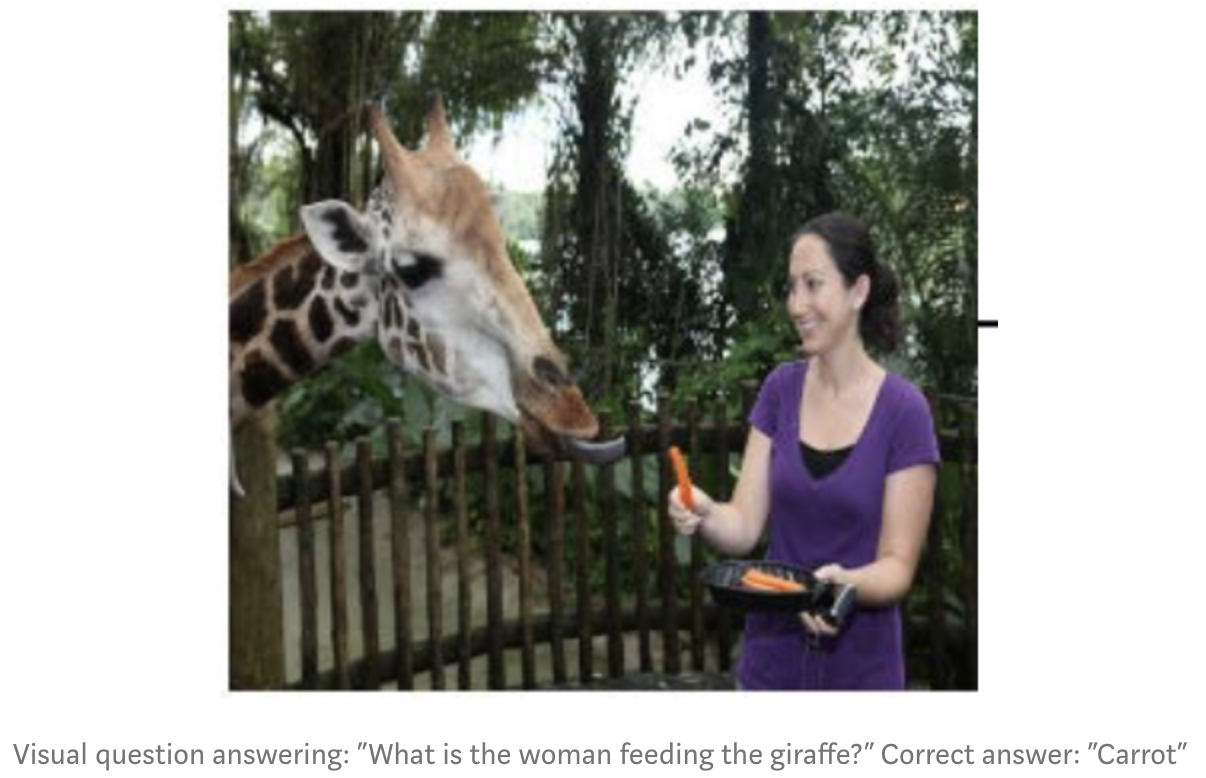
\includegraphics[scale=0.5]{./images/VQA}
\end{center}
\begin{center}
\hspace*{12pt}\hbox{\scriptsize Credit:\thinspace{\itshape \href{https://medium.com/paper-club/multimodal-compact-bilinear-pooling-for-visual-question-answering-and-visual-grounding-6f71bc7d0566}{\color{blue}medium post}\color{black}
}}
\end{center}
\end{frame}
\begin{frame}
\frametitle{Introduction: VG}
\begin{center}
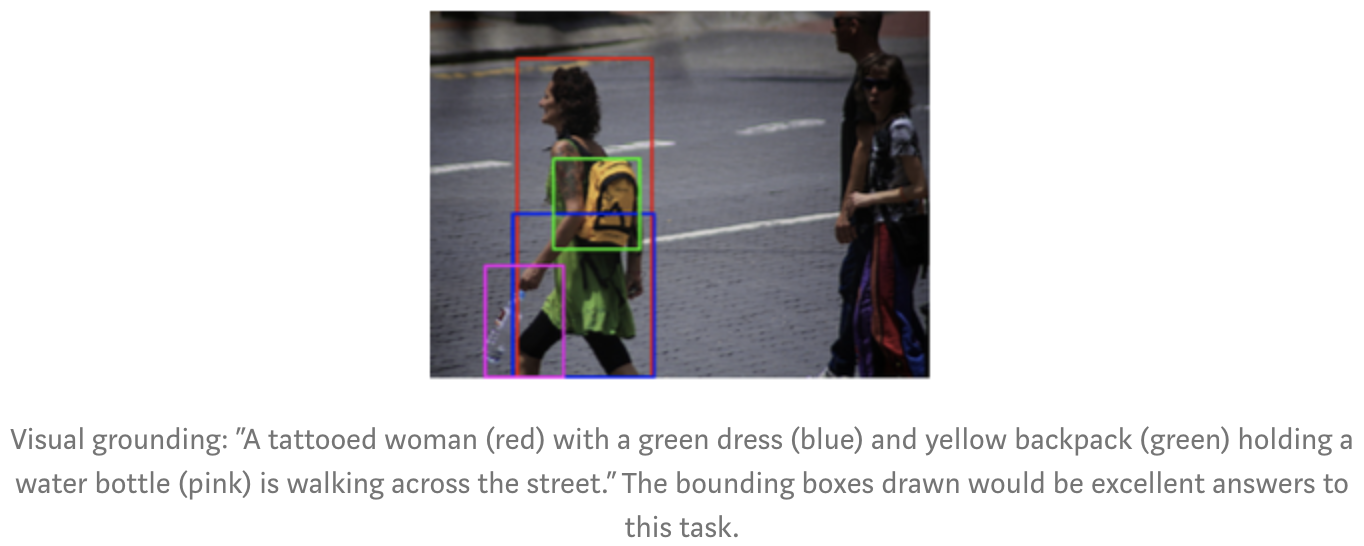
\includegraphics[scale=0.5]{./images/VG}
\end{center}
\begin{center}
\hspace*{12pt}\hbox{\scriptsize Credit:\thinspace{\itshape \href{https://medium.com/paper-club/multimodal-compact-bilinear-pooling-for-visual-question-answering-and-visual-grounding-6f71bc7d0566}{\color{blue}medium post}\color{black}
}}
\end{center}
\end{frame}
\begin{frame}
\frametitle{Introduction}
\begin{center}
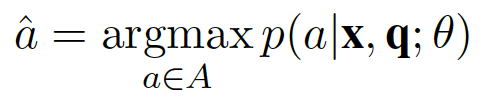
\includegraphics[scale=0.5]{./images/formula01}
\end{center}
\end{frame}

%------------------------------------------------

\subsection{Image encoding}
\begin{frame}
\frametitle{Image encoding}
\begin{center}
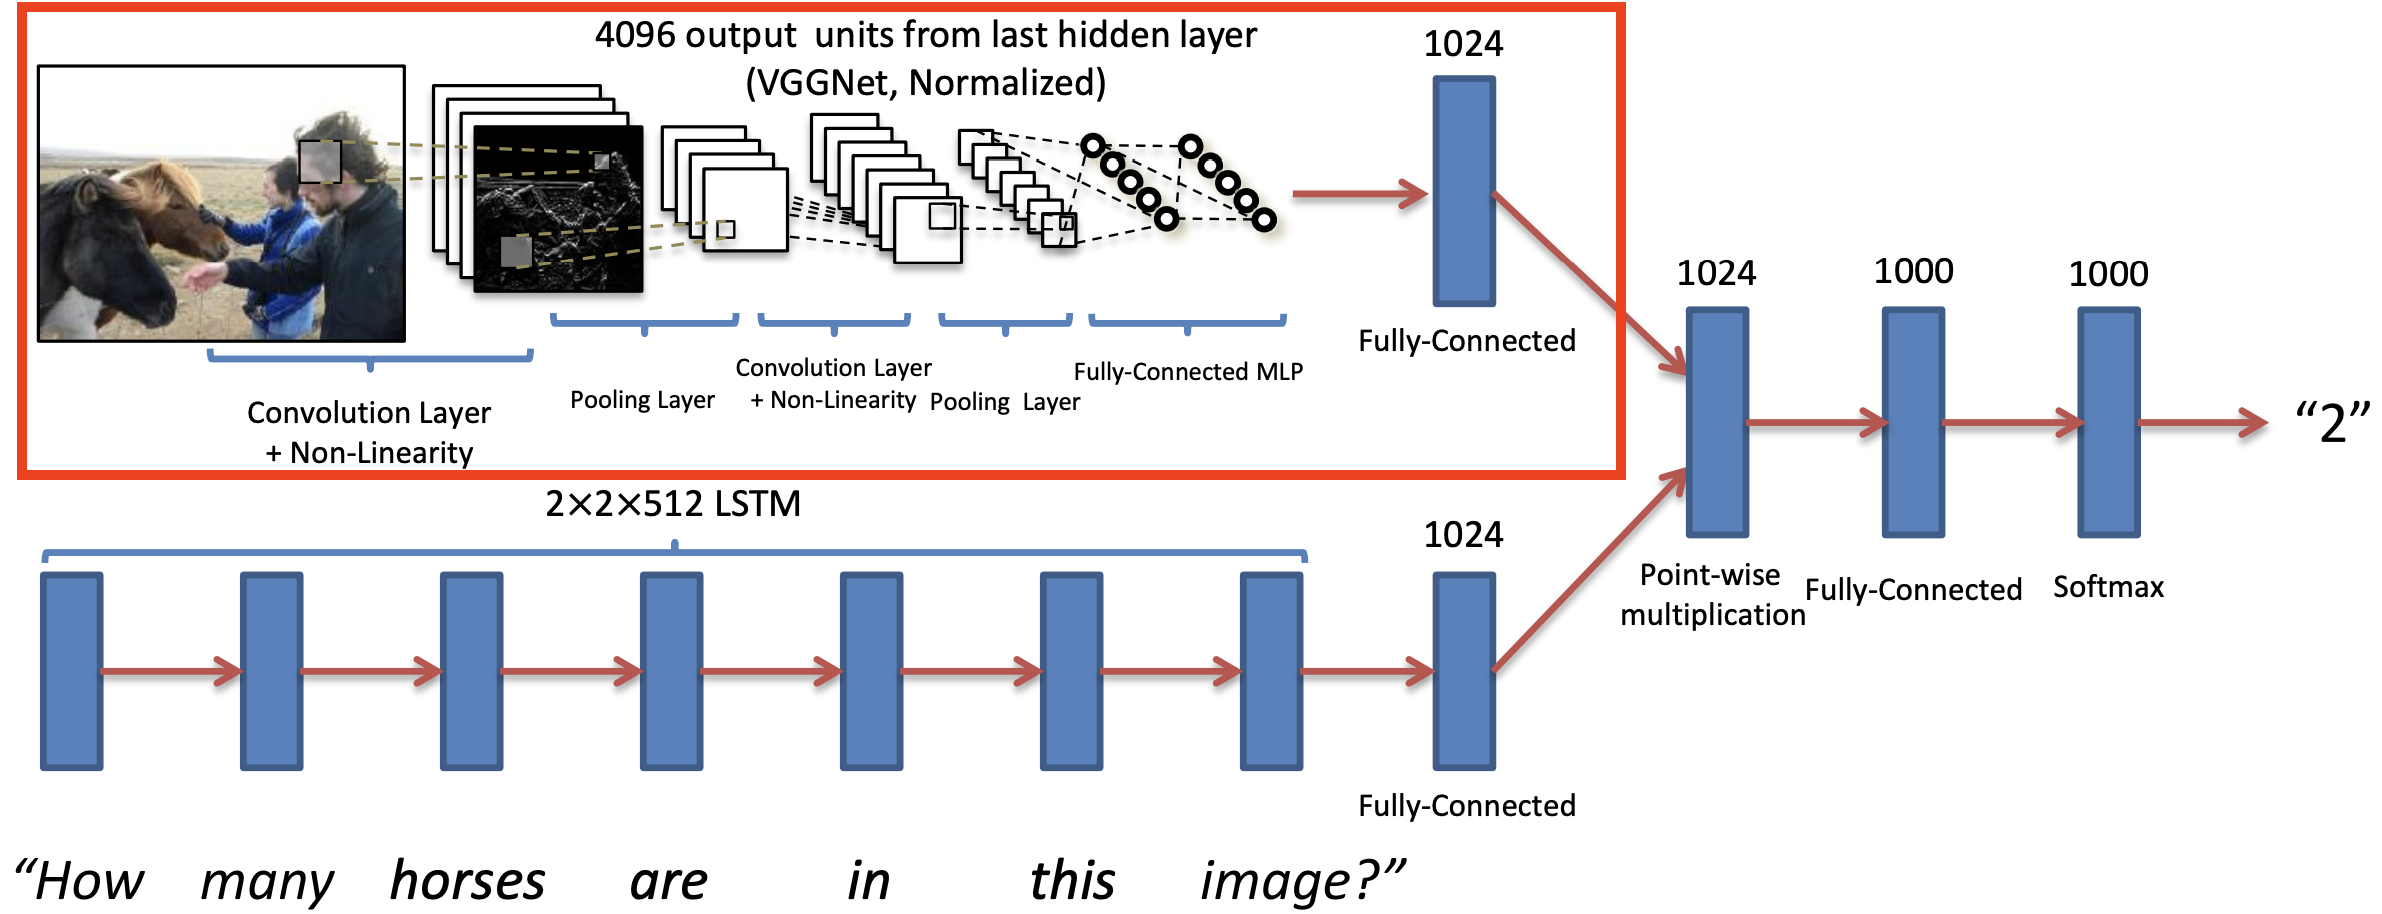
\includegraphics[scale=0.27]{./images/ImageEncoding}
\end{center}
\begin{center}
\hspace*{12pt}\hbox{\scriptsize Credit:\thinspace{\itshape \href{https://arxiv.org/pdf/1505.00468.pdf}{\color{blue}Agrawal et al., 2019}\color{black}
}}
\end{center}
\end{frame}

\subsection{Text encoding}
\begin{frame}
\frametitle{Text encoding}
\begin{center}
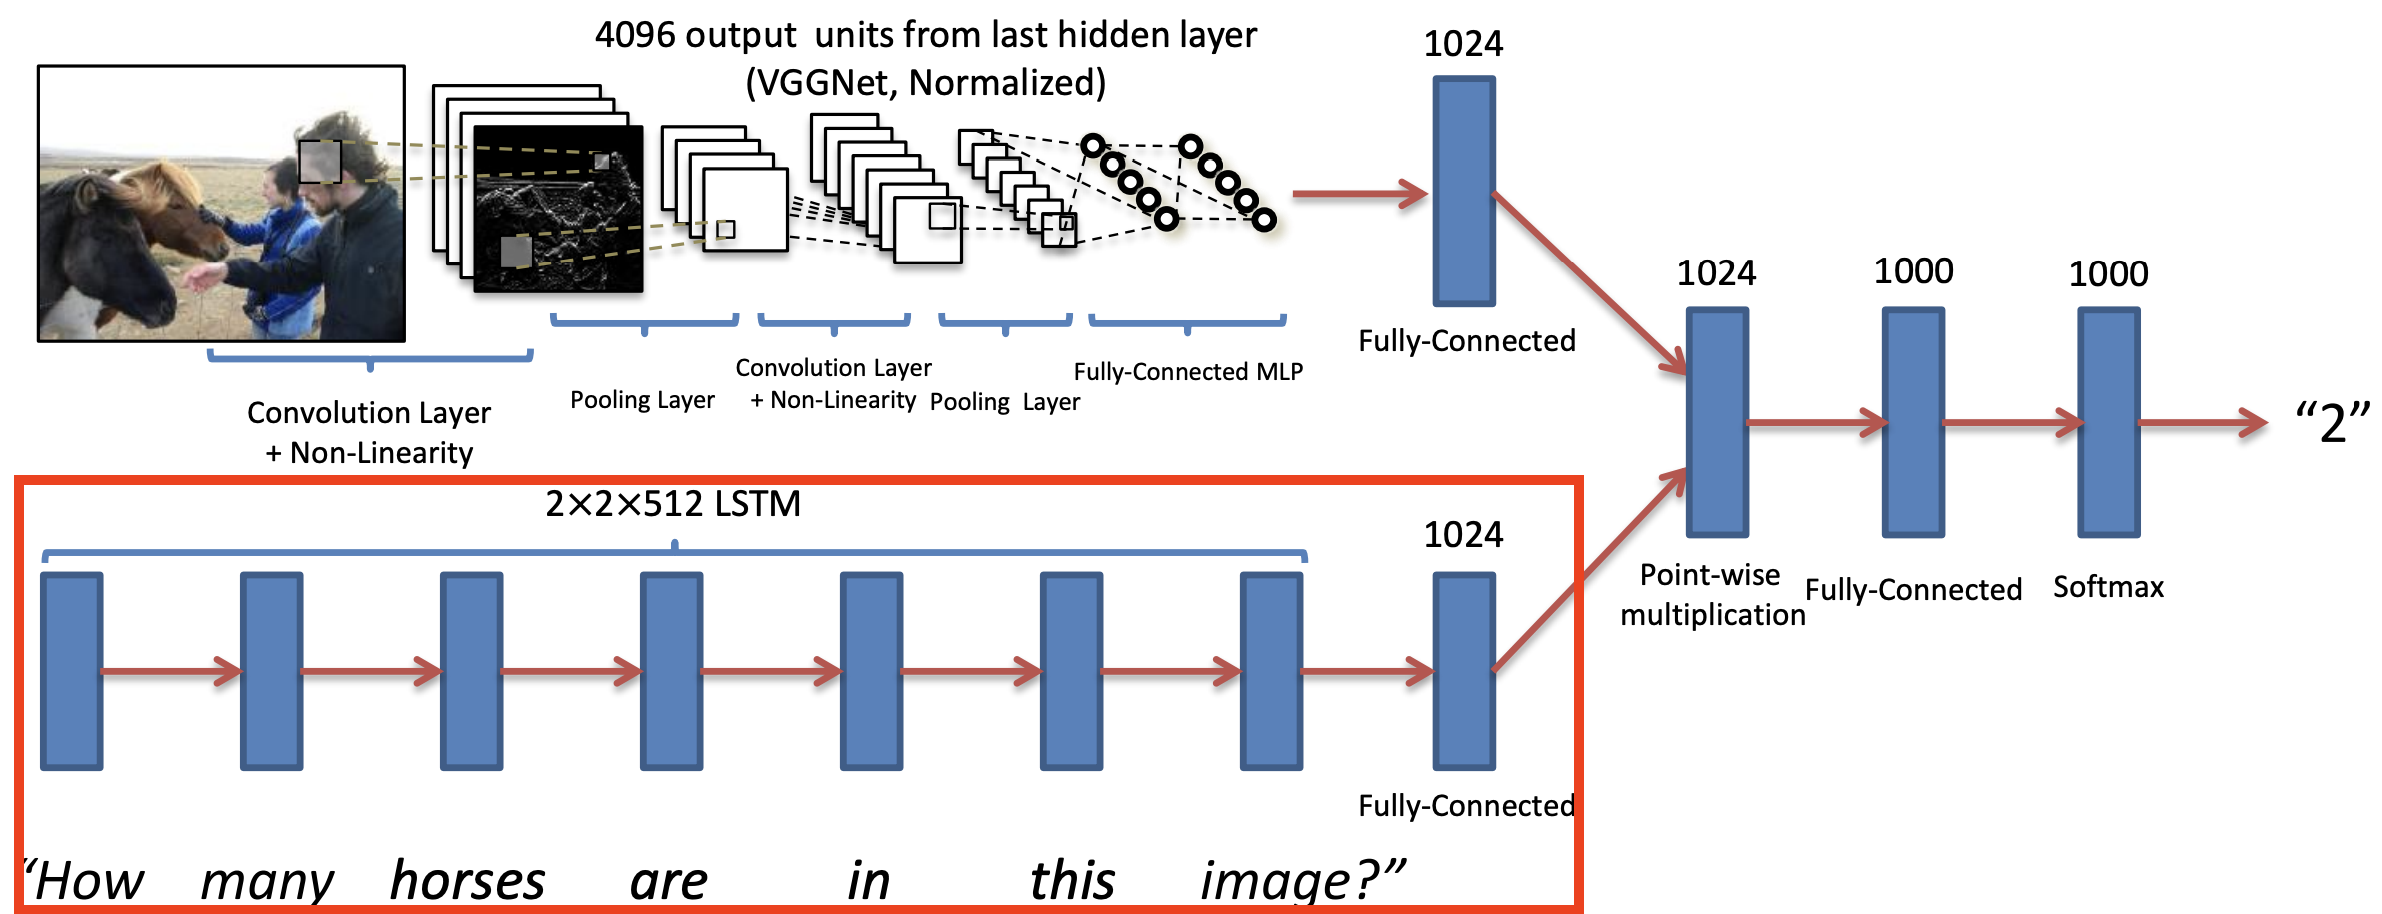
\includegraphics[scale=0.27]{./images/TextEncoding}
\end{center}
\begin{center}
\hspace*{12pt}\hbox{\scriptsize Credit:\thinspace{\itshape \href{https://arxiv.org/pdf/1505.00468.pdf}{\color{blue}Agrawal et al., 2019}\color{black}
}}
\end{center}
\end{frame}

\subsection{Information fusion}
\begin{frame}
\frametitle{Information fusion}
\begin{center}
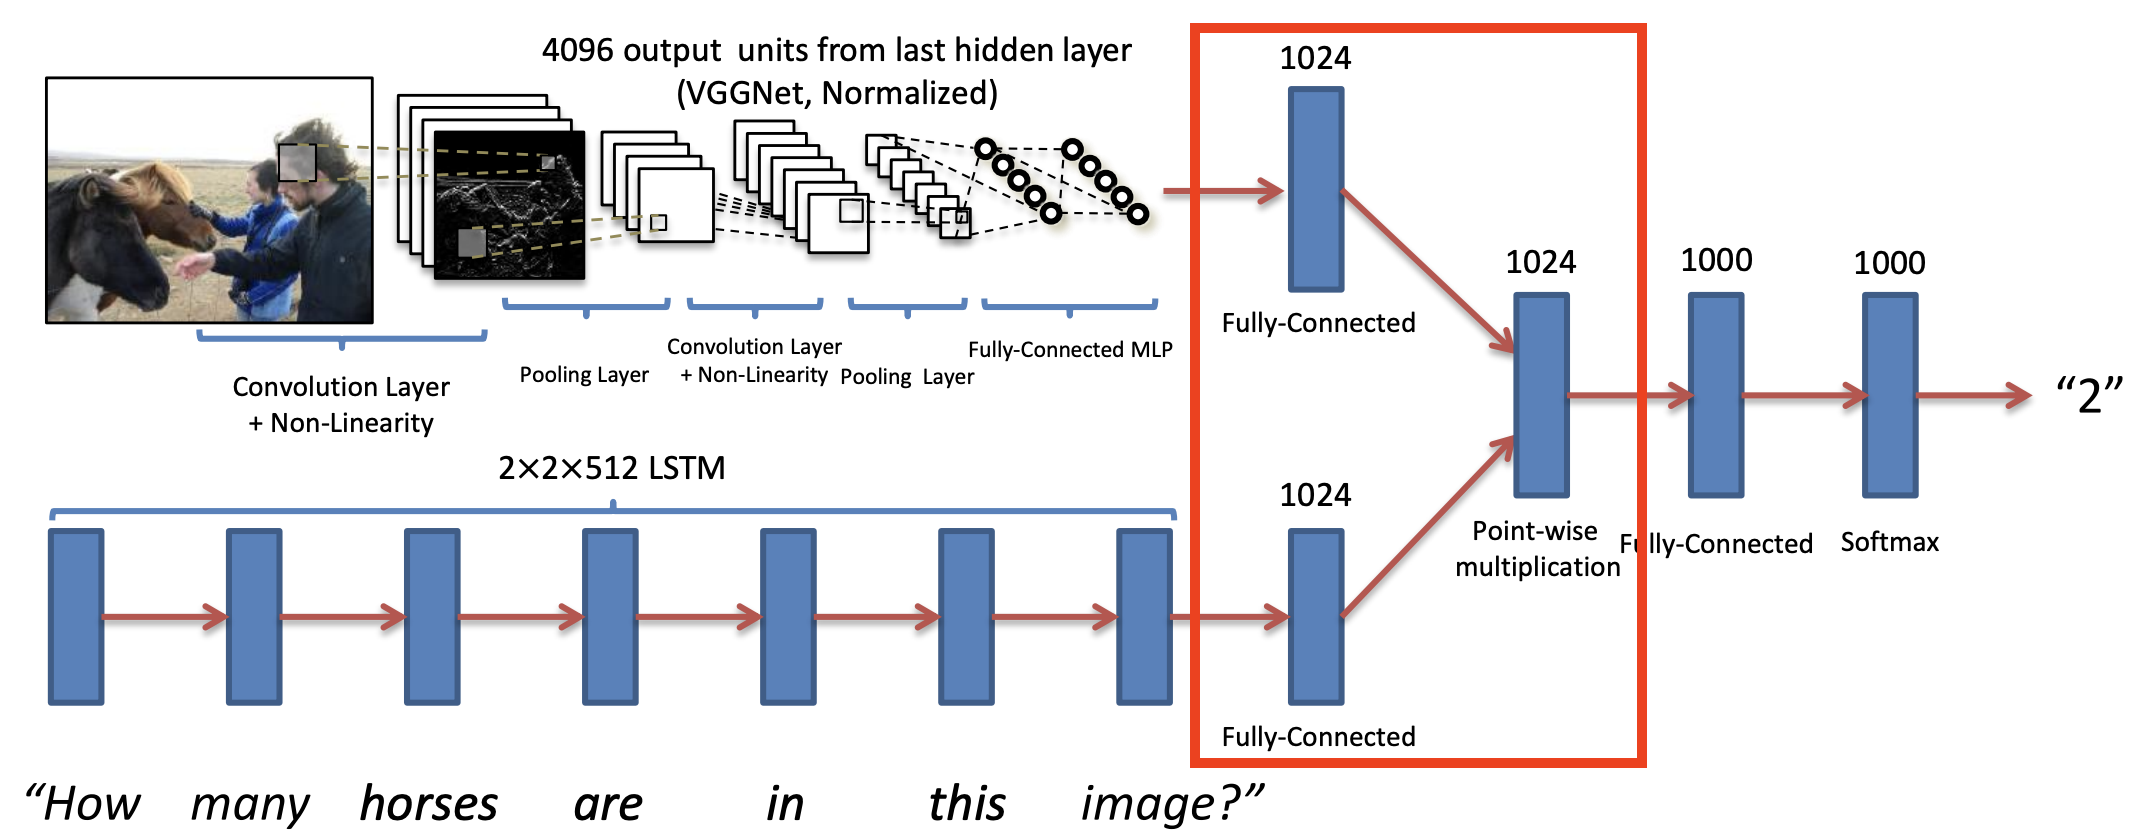
\includegraphics[scale=0.27]{./images/InformationFusion0}
\end{center}
\begin{center}
\hspace*{12pt}\hbox{\scriptsize Credit:\thinspace{\itshape \href{https://arxiv.org/pdf/1505.00468.pdf}{\color{blue}Agrawal et al., 2019}\color{black}
}}
\end{center}
\end{frame}
\begin{frame}
\frametitle{Information fusion}
\begin{center}
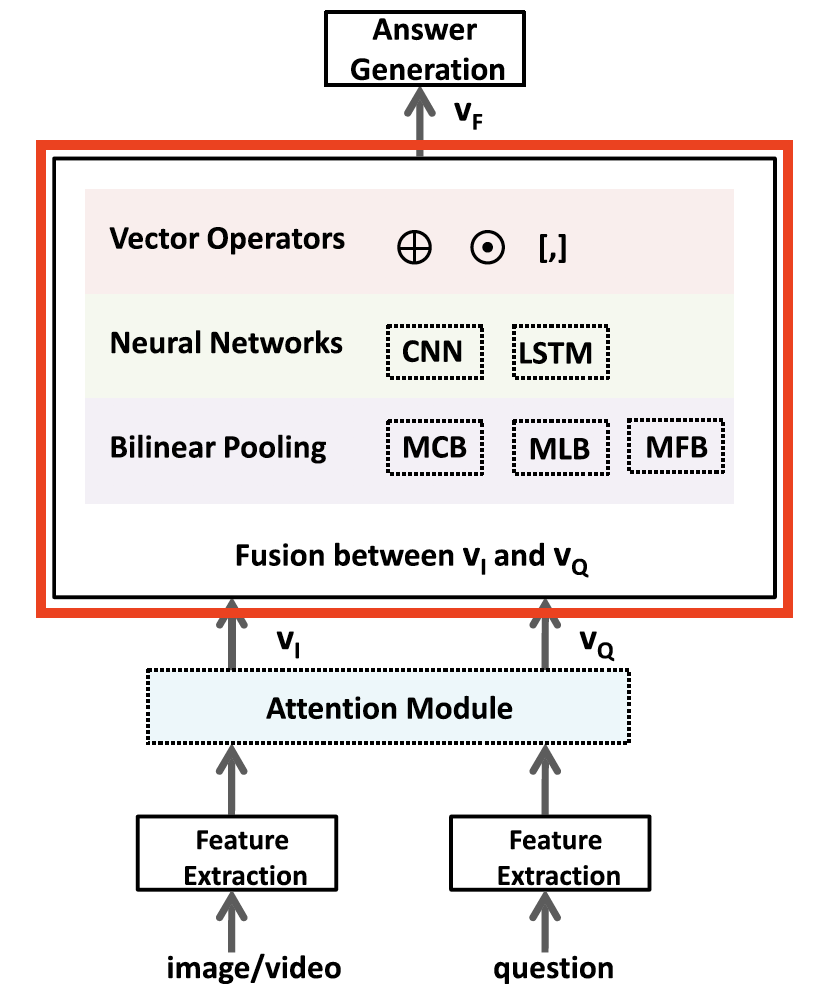
\includegraphics[scale=0.35]{./images/InformationFusion}
\end{center}
\begin{center}
\hspace*{12pt}\hbox{\scriptsize Credit:\thinspace{\itshape \href{https://www.sciencedirect.com/science/article/pii/S1566253518308893}{\color{blue}Zhang et al., 2019}\color{black}
}}
\end{center}
\end{frame}

%------------------------------------------------
%------------------------------------------------

\section{Multimodal Compact Bilinear Pooling} 
\subsection{What is MCB?}
\begin{frame}
\frametitle{What is MCB?}
\textbf{Multimodal Pooling} is combining the two vector representations of image and question (i.e. Multimodal), respectively. This creates a joint representation of the two vectors.

\vspace{0.2cm}

\textbf{Bilinear Pooling} means the outer product of the two input vectors
\begin{itemize}
\item multiply every element of one vector of length N by every element of the other vector of length N, resulting in a matrix of size NxN.
\end{itemize}

\vspace{0.2cm}

\textbf{Compact} bilinear pooling means reducing the dimensionality to get almost the same level of power with way fewer parameters.

\end{frame}

\begin{frame}
\frametitle{What is MCB?}
\begin{center}
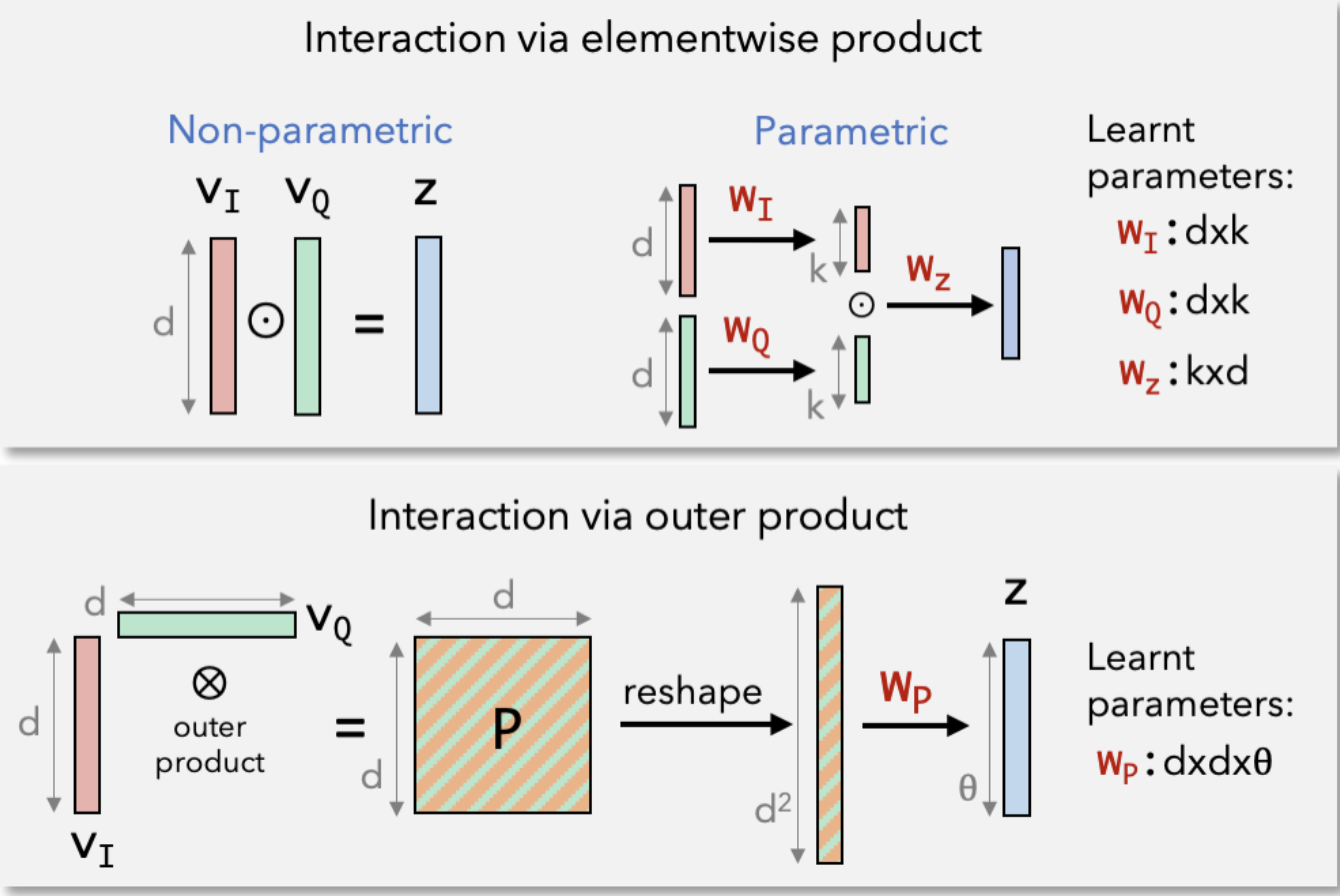
\includegraphics[scale=0.42]{./images/imfus.png}
\end{center}
\begin{center}
\hspace*{12pt}\hbox{\scriptsize Credit:\thinspace{\itshape \href{https://medium.com/ai2-blog/the-lure-of-the-outer-product-4addd2e7f95e}{\color{blue}The lure of the outer product}\color{black}
}}
\end{center}
\end{frame}

%------------------------------------------------

\subsection{Why MCB?}

\begin{frame}
\frametitle{Why MCB?}
\begin{itemize}
\item Vector operations are too simplistic to fully capture the relationships between images and text
\item So many non-linear neural networks to learn the interaction between the visual and textual features
\item Research like \href{https://www.sciencedirect.com/science/article/pii/S1566253518308893}{\color{blue}Zhang et al., 2019} \color{black}confirm that Bilinear Pooling is the promising road to take for information fusion
\item Bilinear pooling is a very rich representation that allows a full multiplicative interaction between all elements of both vectors capturing any possible relationship
\item However, in bilinear pooling  the number of resulting parameters is too high to be practical. For example,
\begin{itemize}
\item if the image and text vectors are of length 2048
\item the resulting matrix would have \begin{math}2048^{2}\end{math} elements
\item and we’d need to fully connect that matrix to 3000 classes
\item it results in \begin{math}~\end{math}12.5 billion learnable parameters
\end{itemize}
\item Therefore, introducing MCB to capture the discriminating abilities of bilinear pooling with only a a few thousand parameters (16k)
\end{itemize}
\end{frame}

%------------------------------------------------

\subsection{How to MCB?}
\begin{frame}
\frametitle{How to MCB?}
\begin{center}
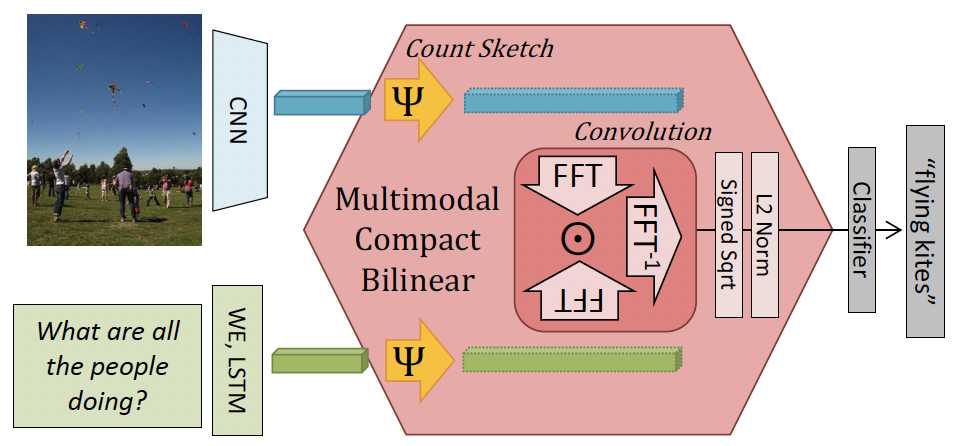
\includegraphics[scale=0.5]{./images/How_to_MCB01}
\end{center}
\end{frame}
\begin{frame}
\frametitle{How to MCB?}
\begin{center}
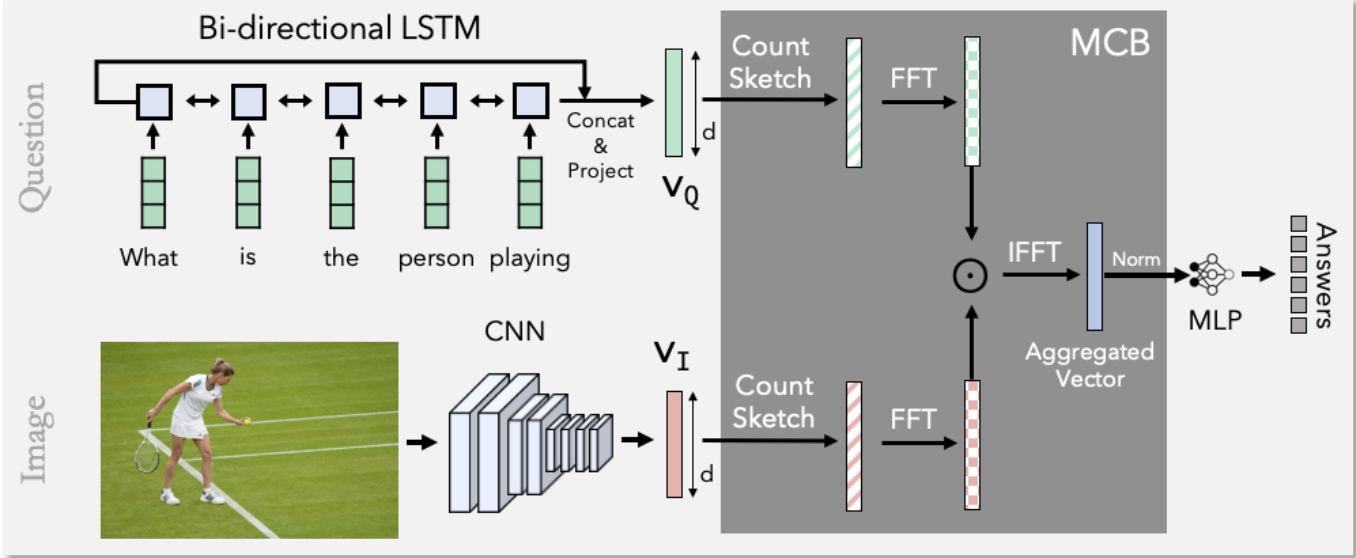
\includegraphics[scale=0.5]{./images/mcb}
\end{center}
\begin{center}
\hspace*{12pt}\hbox{\scriptsize Credit:\thinspace{\itshape \href{https://medium.com/ai2-blog/the-lure-of-the-outer-product-4addd2e7f95e}{\color{blue}The lure of the outer product}\color{black}
}}
\end{center}
\end{frame}
\begin{frame}
\frametitle{How to MCB?}
MCB is approximated by
\begin{itemize}
\item randomly projecting the image and text representations to a \color{black}higher \color{black} dimensional space using Count Sketch
\item and then convolving both vectors efficiently by using element-wise product in FFT space
\item $z = w[x \otimes q]$
\item about 12.5 billion parameters for 2048 images and texts and 3000 classes!
\end{itemize}
MCB key feature
\begin{itemize}
\item using Count Sketch over outer product to use convolution, and FFT
\begin{itemize}
\item projecting the outer product to a lower dimensional space
\item avoiding computing the outer product directly:
\begin{itemize}
\item $\Psi(x \otimes q, h, s) = \Psi(x, h, s) * \Psi(q, h, s) $
\end{itemize}
\end{itemize}
\end{itemize}
\end{frame}
\begin{frame}
\frametitle{How to MCB?}
%\begin{center}
%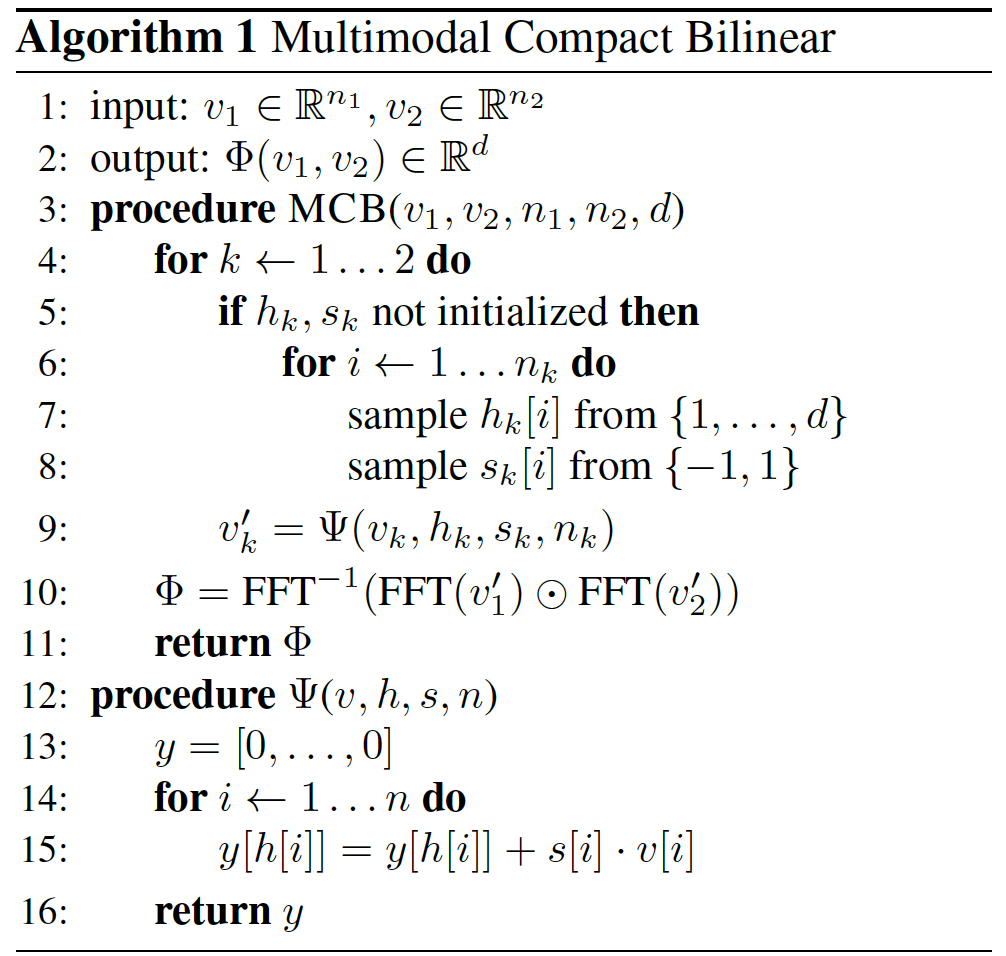
\includegraphics[scale=0.45]{./images/How_to_MCB0201}
%\end{center}
\begin{figure}%
    \centering
    %\subfloat[]{{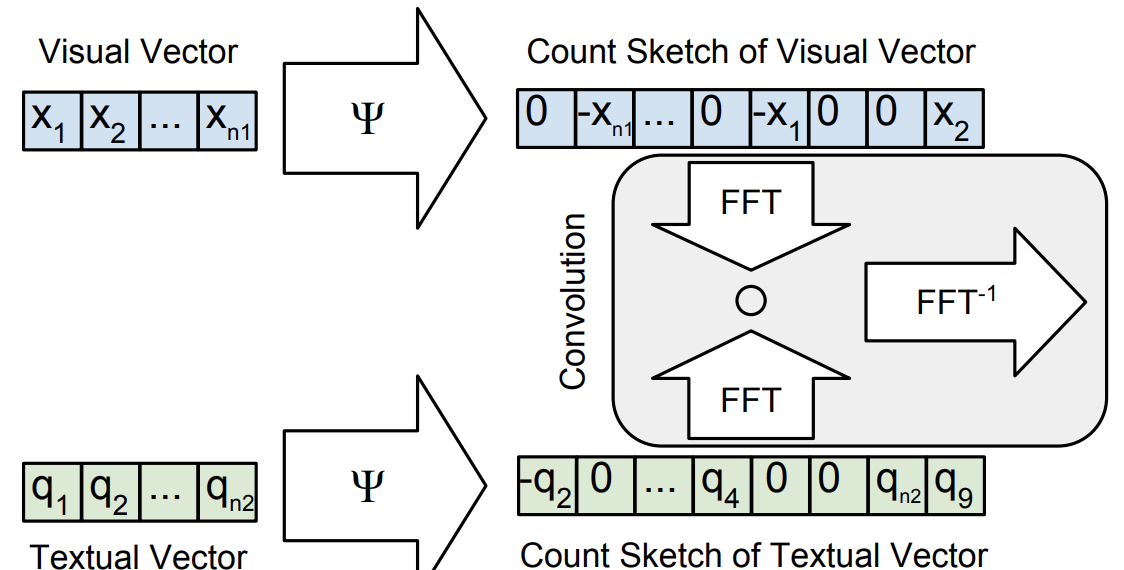
\includegraphics[width=5cm]{./images/How_to_MCB0202} }}%
    {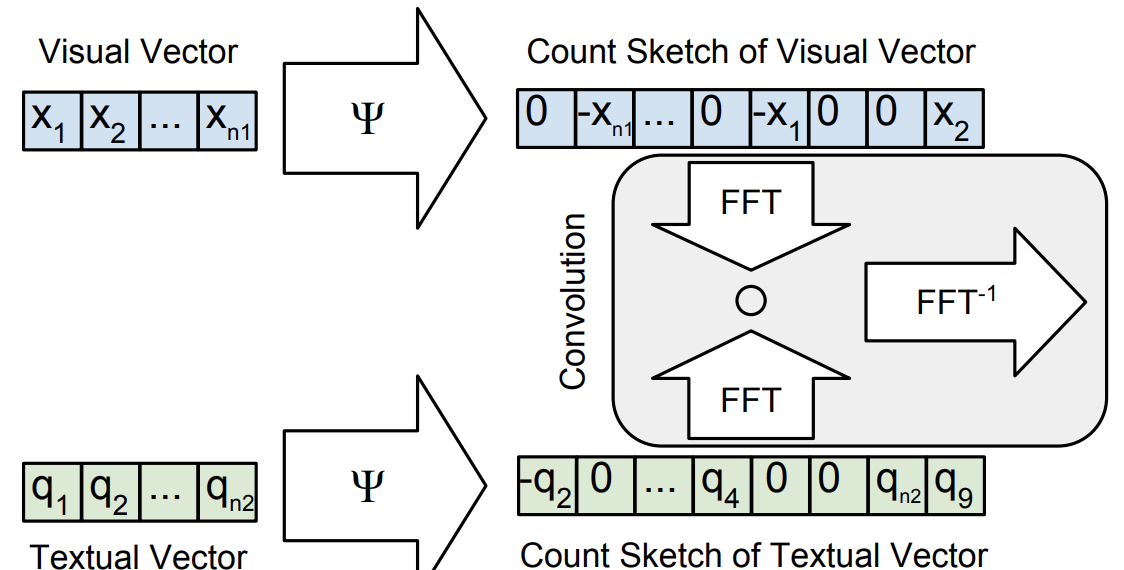
\includegraphics[width=5cm]{./images/How_to_MCB0202} }%
    \qquad
    {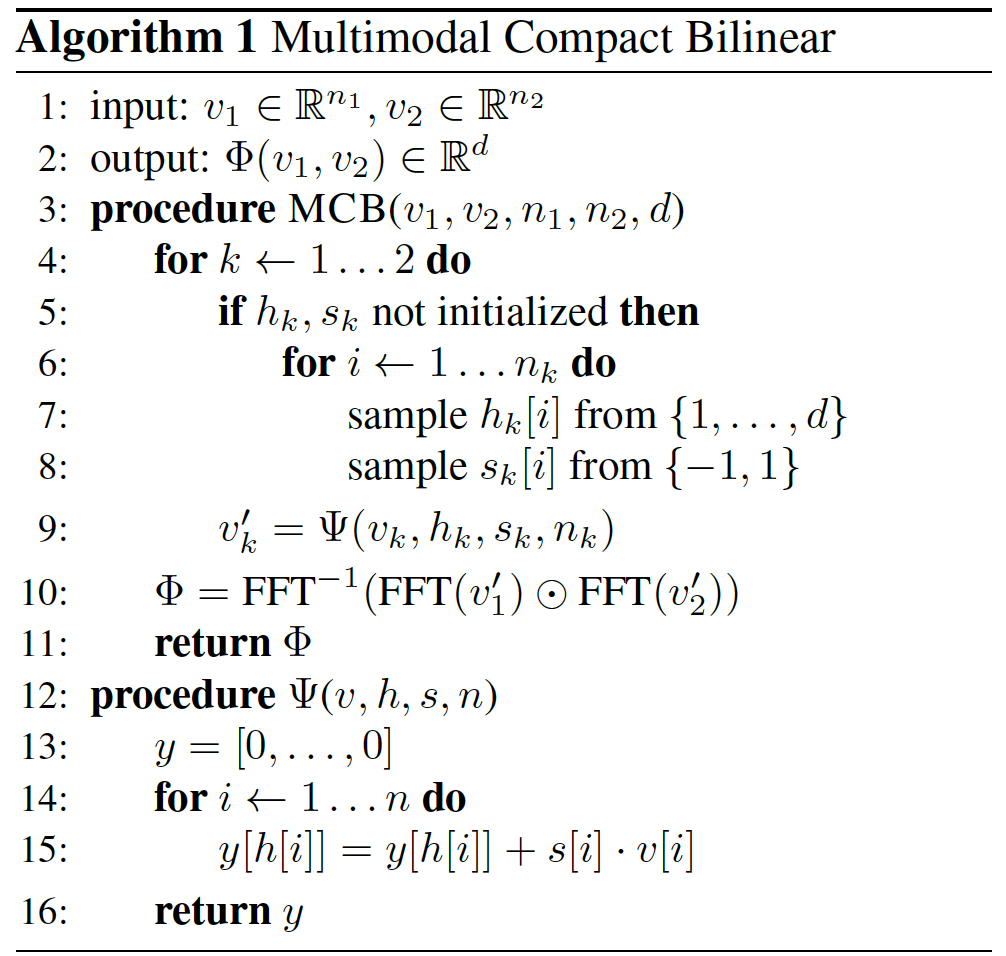
\includegraphics[width=5cm]{./images/How_to_MCB0201} }%
    %\caption{}%
    \label{fig:example}%
\end{figure}
\end{frame}
%\begin{frame}
%\frametitle{How to MCB?}
%MCB is used at three different points where visual and textual representations need to be combined
%\begin{enumerate} 
%  \item to predict spatial attention in the image 
%  \item to predict an answer to the question
%  \item to relate the encoded multiple-choice answers to the combined question+image space (this only applies to the multiple choice problem)
%  \end{enumerate}  
% 
% \vspace{0.3cm}
% 
%They also use attention maps and additional training data, which feels a bit like sacrificing experimental purity to achieve state-of-the-art results.
%\end{frame}
\begin{frame}
\frametitle{Attention models}
Attention models use an attention score between the question and each region in the image. The resulting attention vector helps the model to focus on the most relevant region(s) in the image to answer the given question.
\end{frame}
\begin{frame}
\frametitle{How to MCB?}
\begin{center}
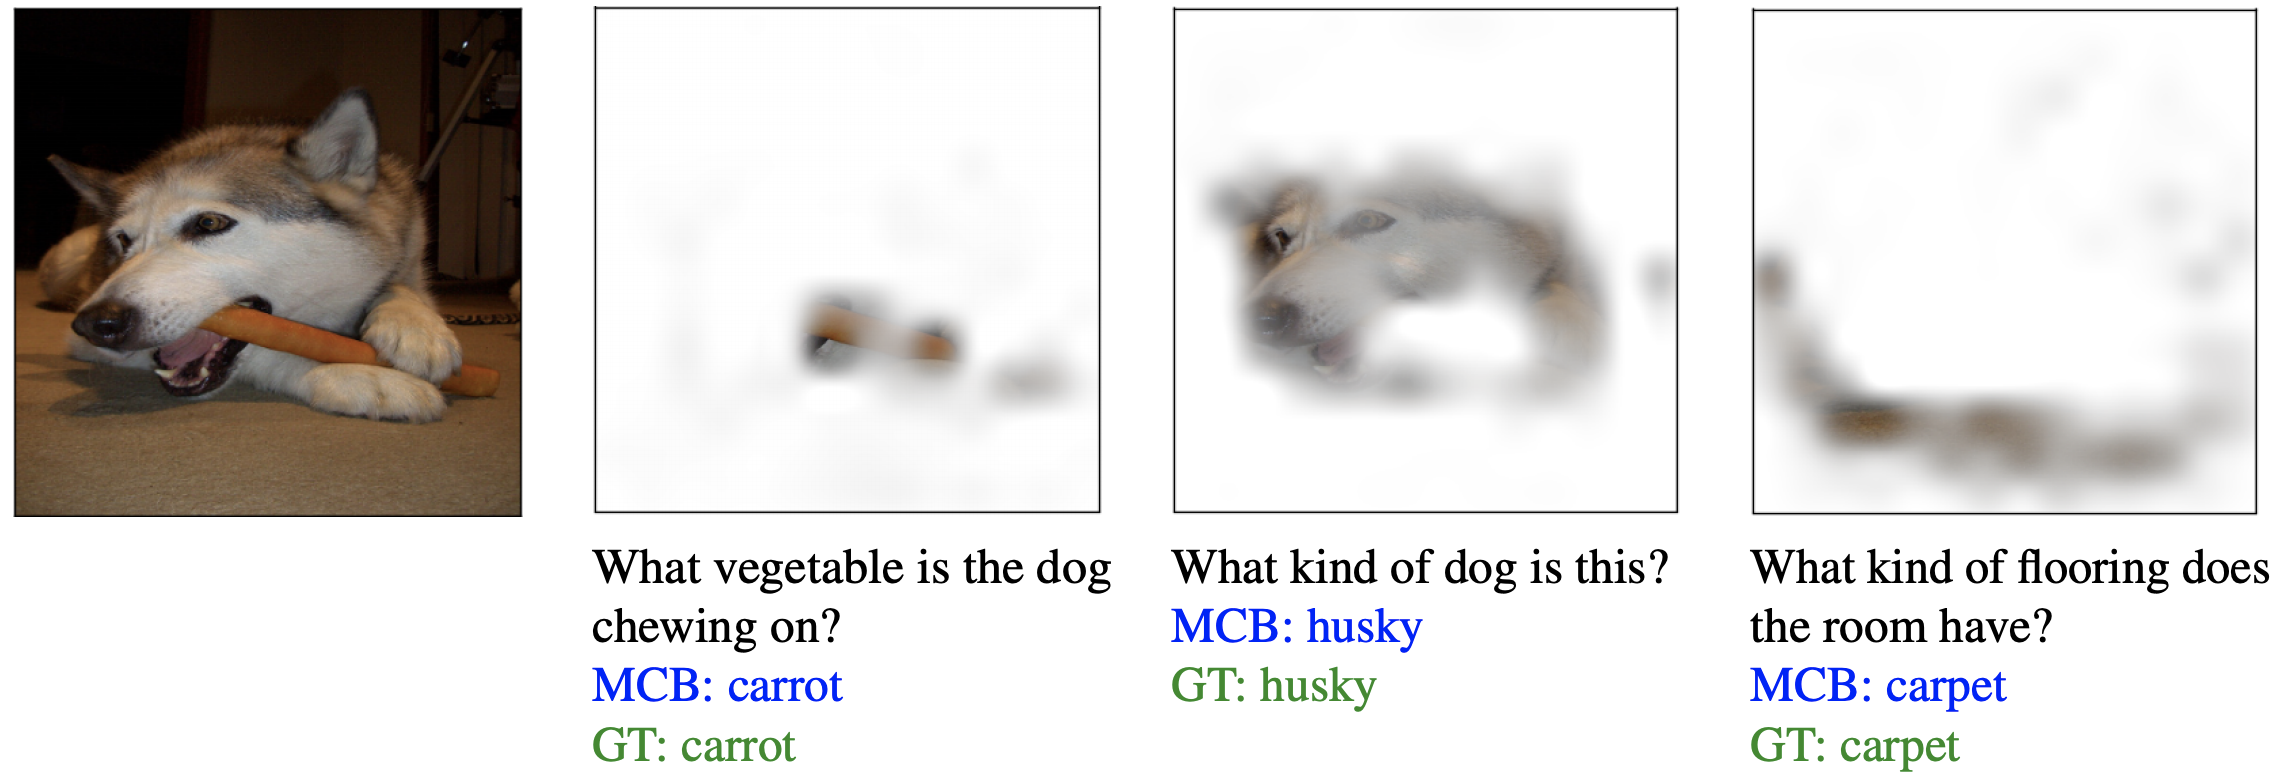
\includegraphics[scale=0.3]{./images/attention}
\end{center}
\end{frame}
\begin{frame}
\frametitle{How to MCB?}
\begin{center}
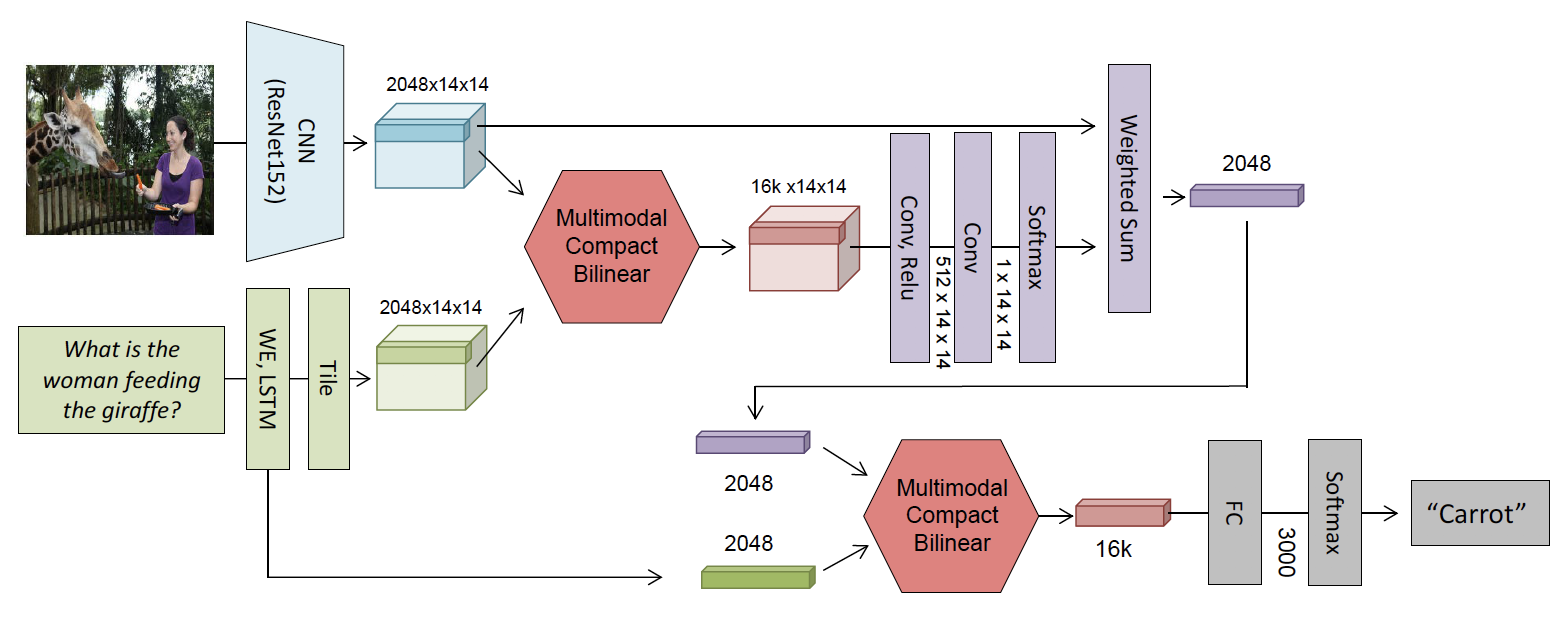
\includegraphics[scale=0.45]{./images/How_to_MCB03}
\end{center}
\end{frame}

%------------------------------------------------

\subsection{Architecture of MCB}
\begin{frame}
\frametitle{Architecture of MCB}
\begin{center}
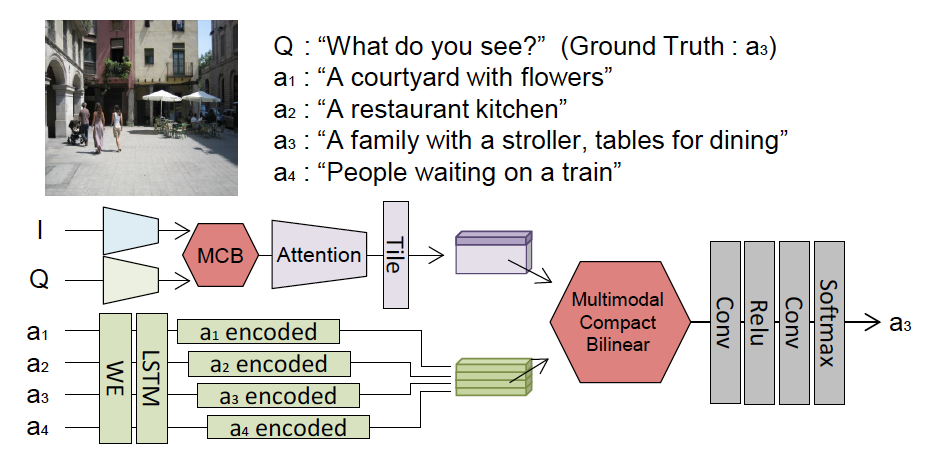
\includegraphics[scale=0.65]{./images/MCB_Architecture01}
\end{center}
\end{frame}
\begin{frame}
\frametitle{Architecture of MCB}
\begin{center}
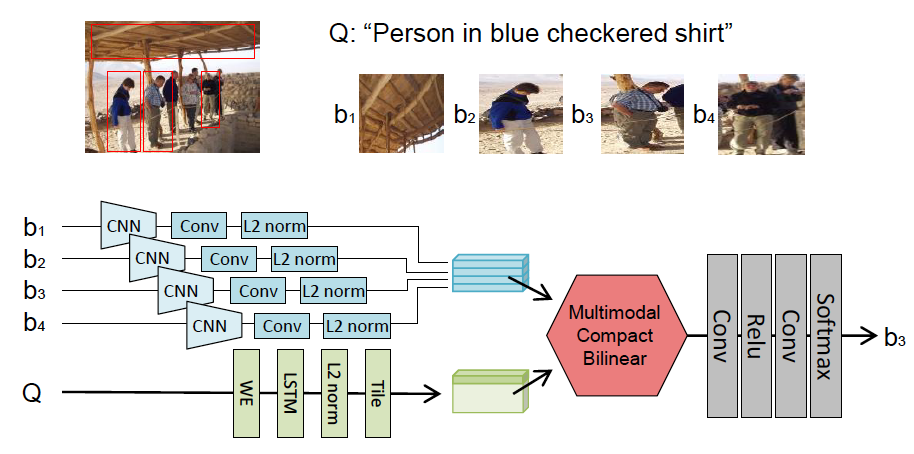
\includegraphics[scale=0.65]{./images/MCB_Architecture02}
\end{center}
\end{frame}
%------------------------------------------------
%------------------------------------------------

\section{Experiments and Results} 
\subsection{Datasets}
\begin{frame}
\frametitle{Datasets}
For Visual Question Answering
\begin{enumerate} 
  \item MSCOCO
  \item Visual Genome
  \item Visual7W
  \end{enumerate}  
  
   \vspace{0.5cm}

  
For Visual Grounding
  \begin{enumerate} 
  \item Flickr30k
  \item ReflectItGame
  \end{enumerate} 
\end{frame}
%------------------------------------------------

\subsection{VQA}
\begin{frame}
\frametitle{VQA}
\begin{center}
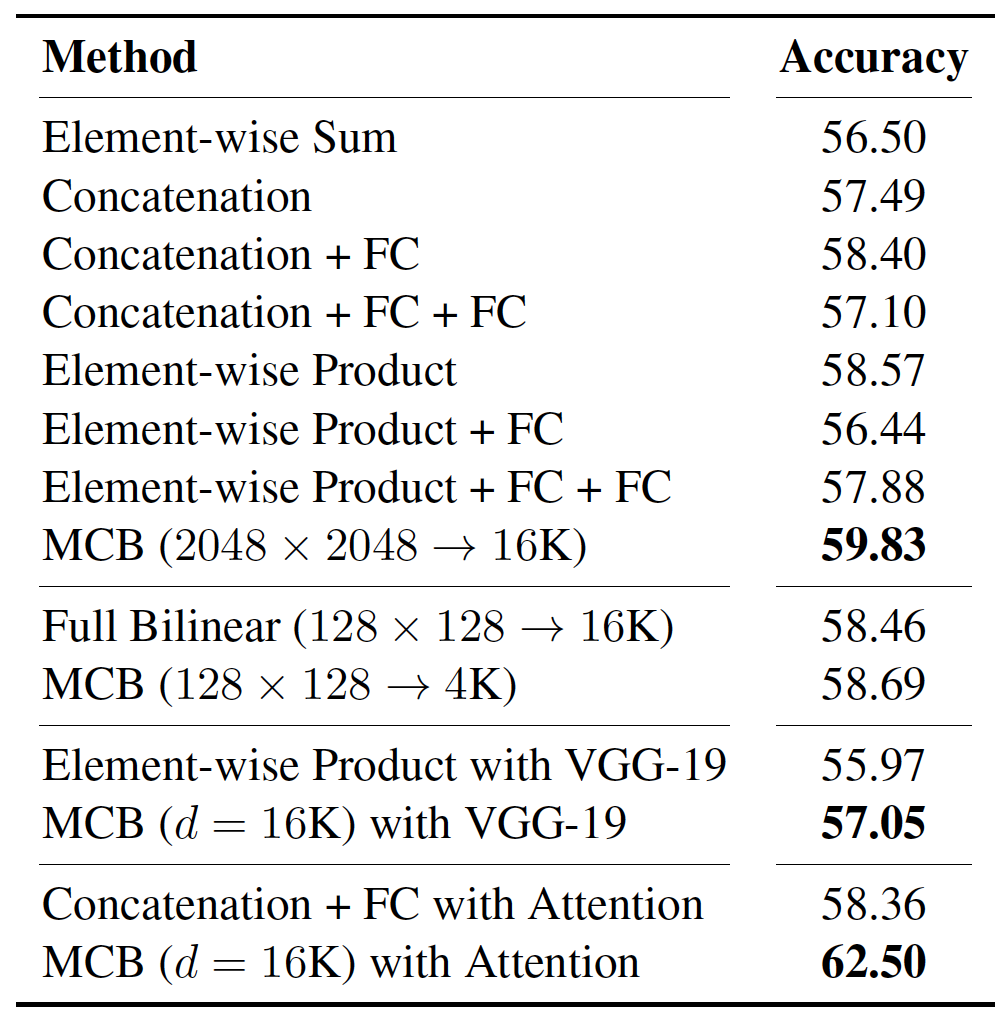
\includegraphics[scale=0.4]{./images/VQA_Result01}
\end{center}
\end{frame}
\begin{frame}
\frametitle{VQA}
\begin{center}
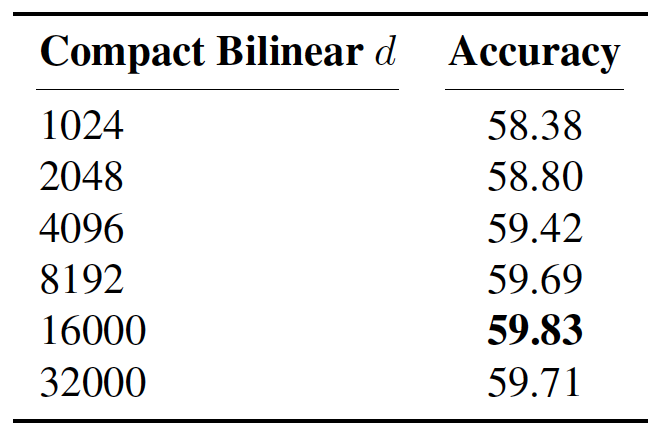
\includegraphics[scale=0.5]{./images/VQA_Result02}
\end{center}
\end{frame}
\begin{frame}
\frametitle{VQA}
\begin{center}
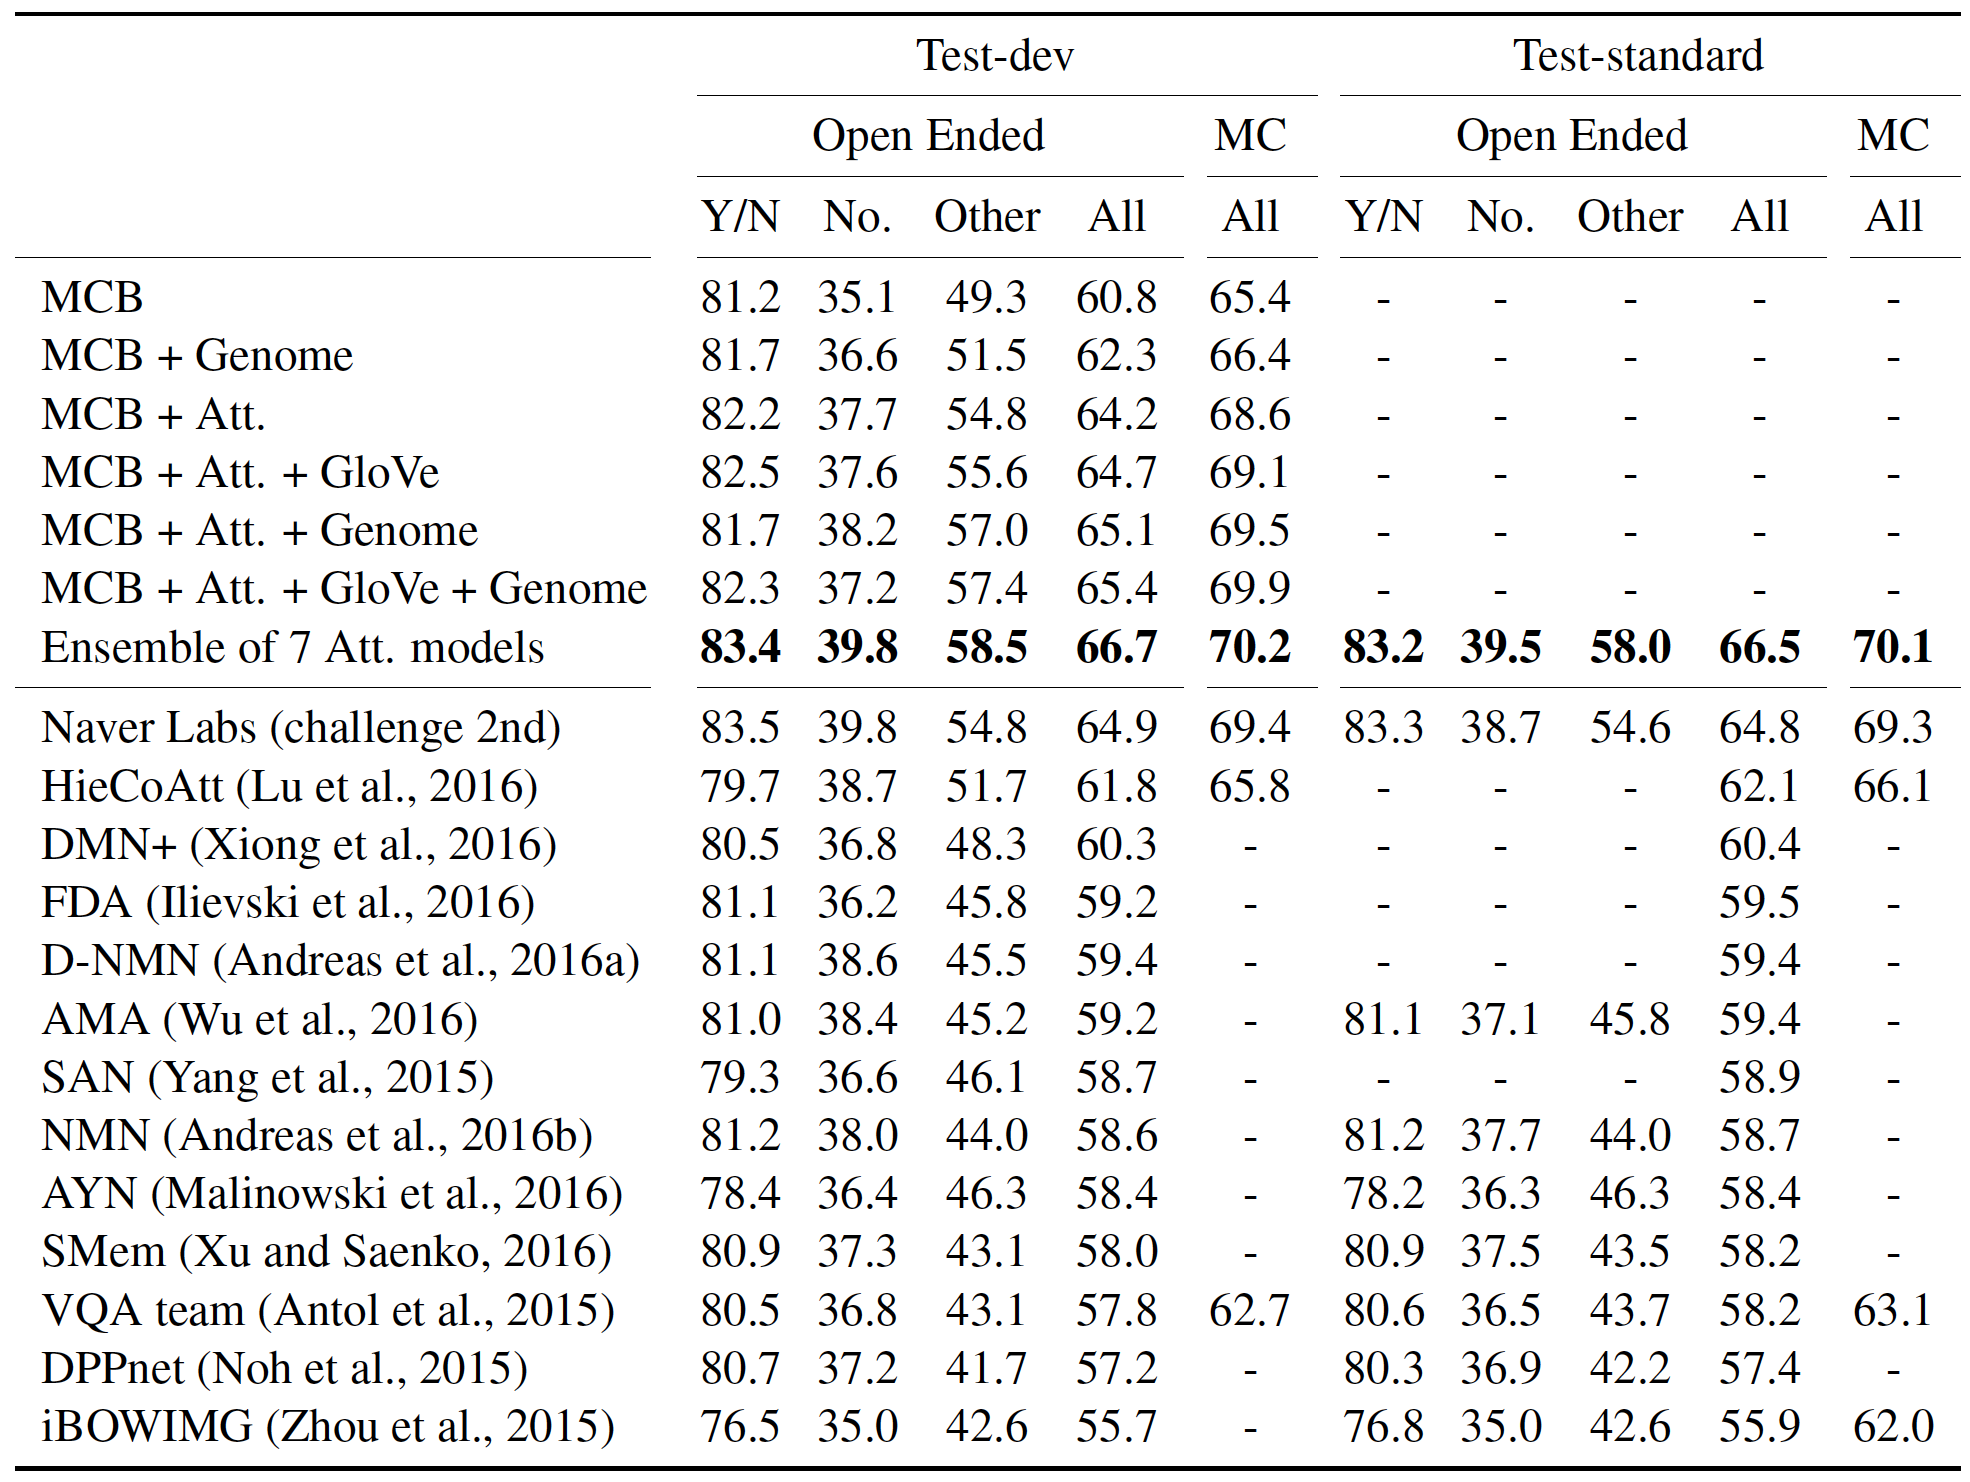
\includegraphics[scale=0.3]{./images/VQA_Result03}
\end{center}
\end{frame}
\begin{frame}
\frametitle{VQA}
\begin{center}
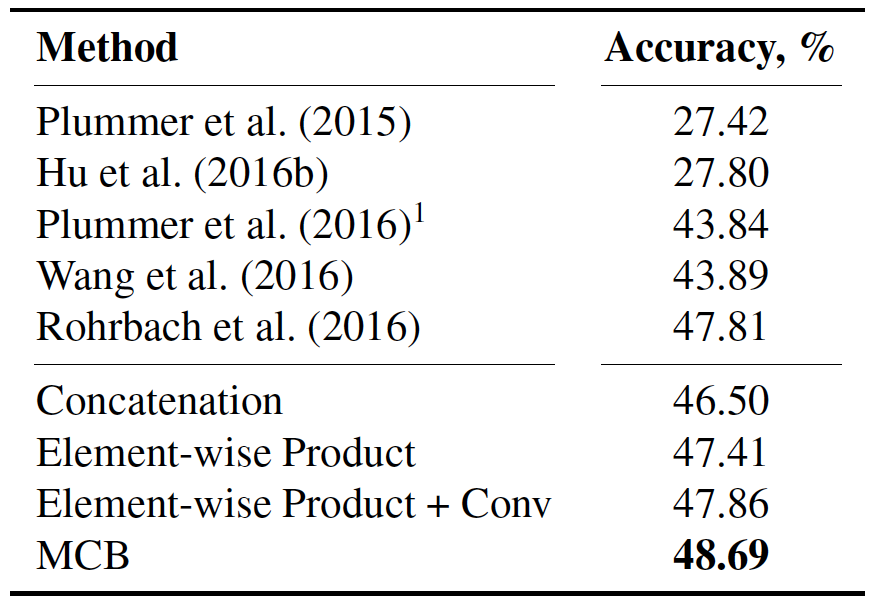
\includegraphics[scale=0.5]{./images/VQA_Result04}
\end{center}
\end{frame}
\begin{frame}
\frametitle{VQA}
\begin{center}
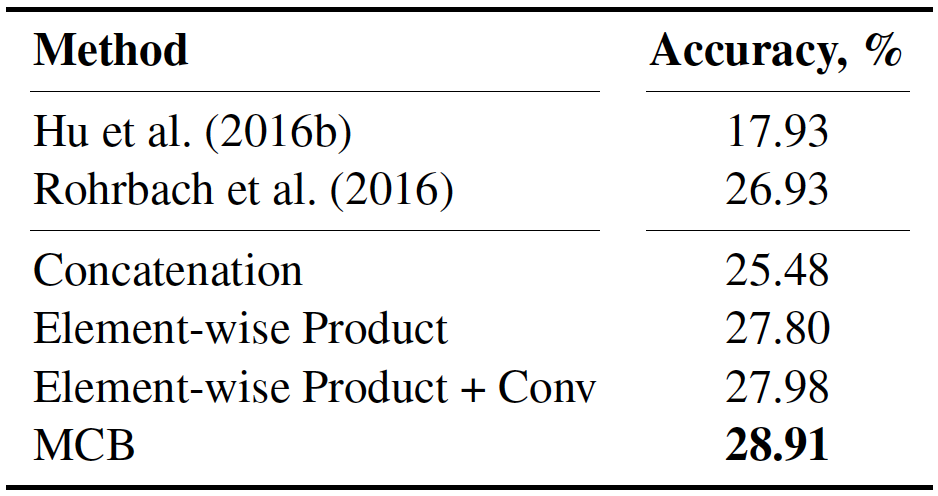
\includegraphics[scale=0.5]{./images/VQA_Result05}
\end{center}
\end{frame}
%------------------------------------------------

\subsection{Visual Grounding}
\begin{frame}
\frametitle{Visual Grounding}
\begin{center}
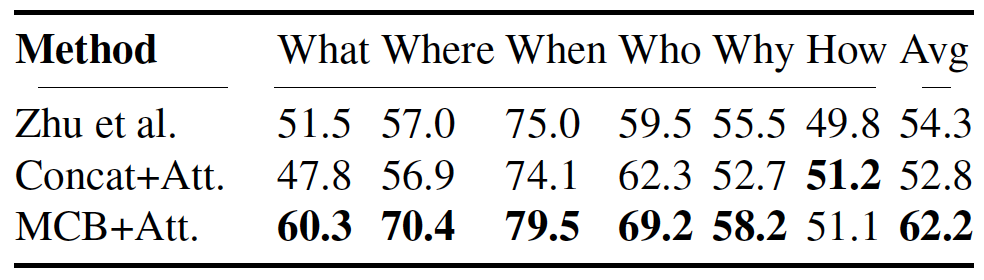
\includegraphics[scale=0.5]{./images/VG_Result01}
\end{center}
\end{frame}
\begin{frame}
\frametitle{Visual Grounding}
\begin{center}
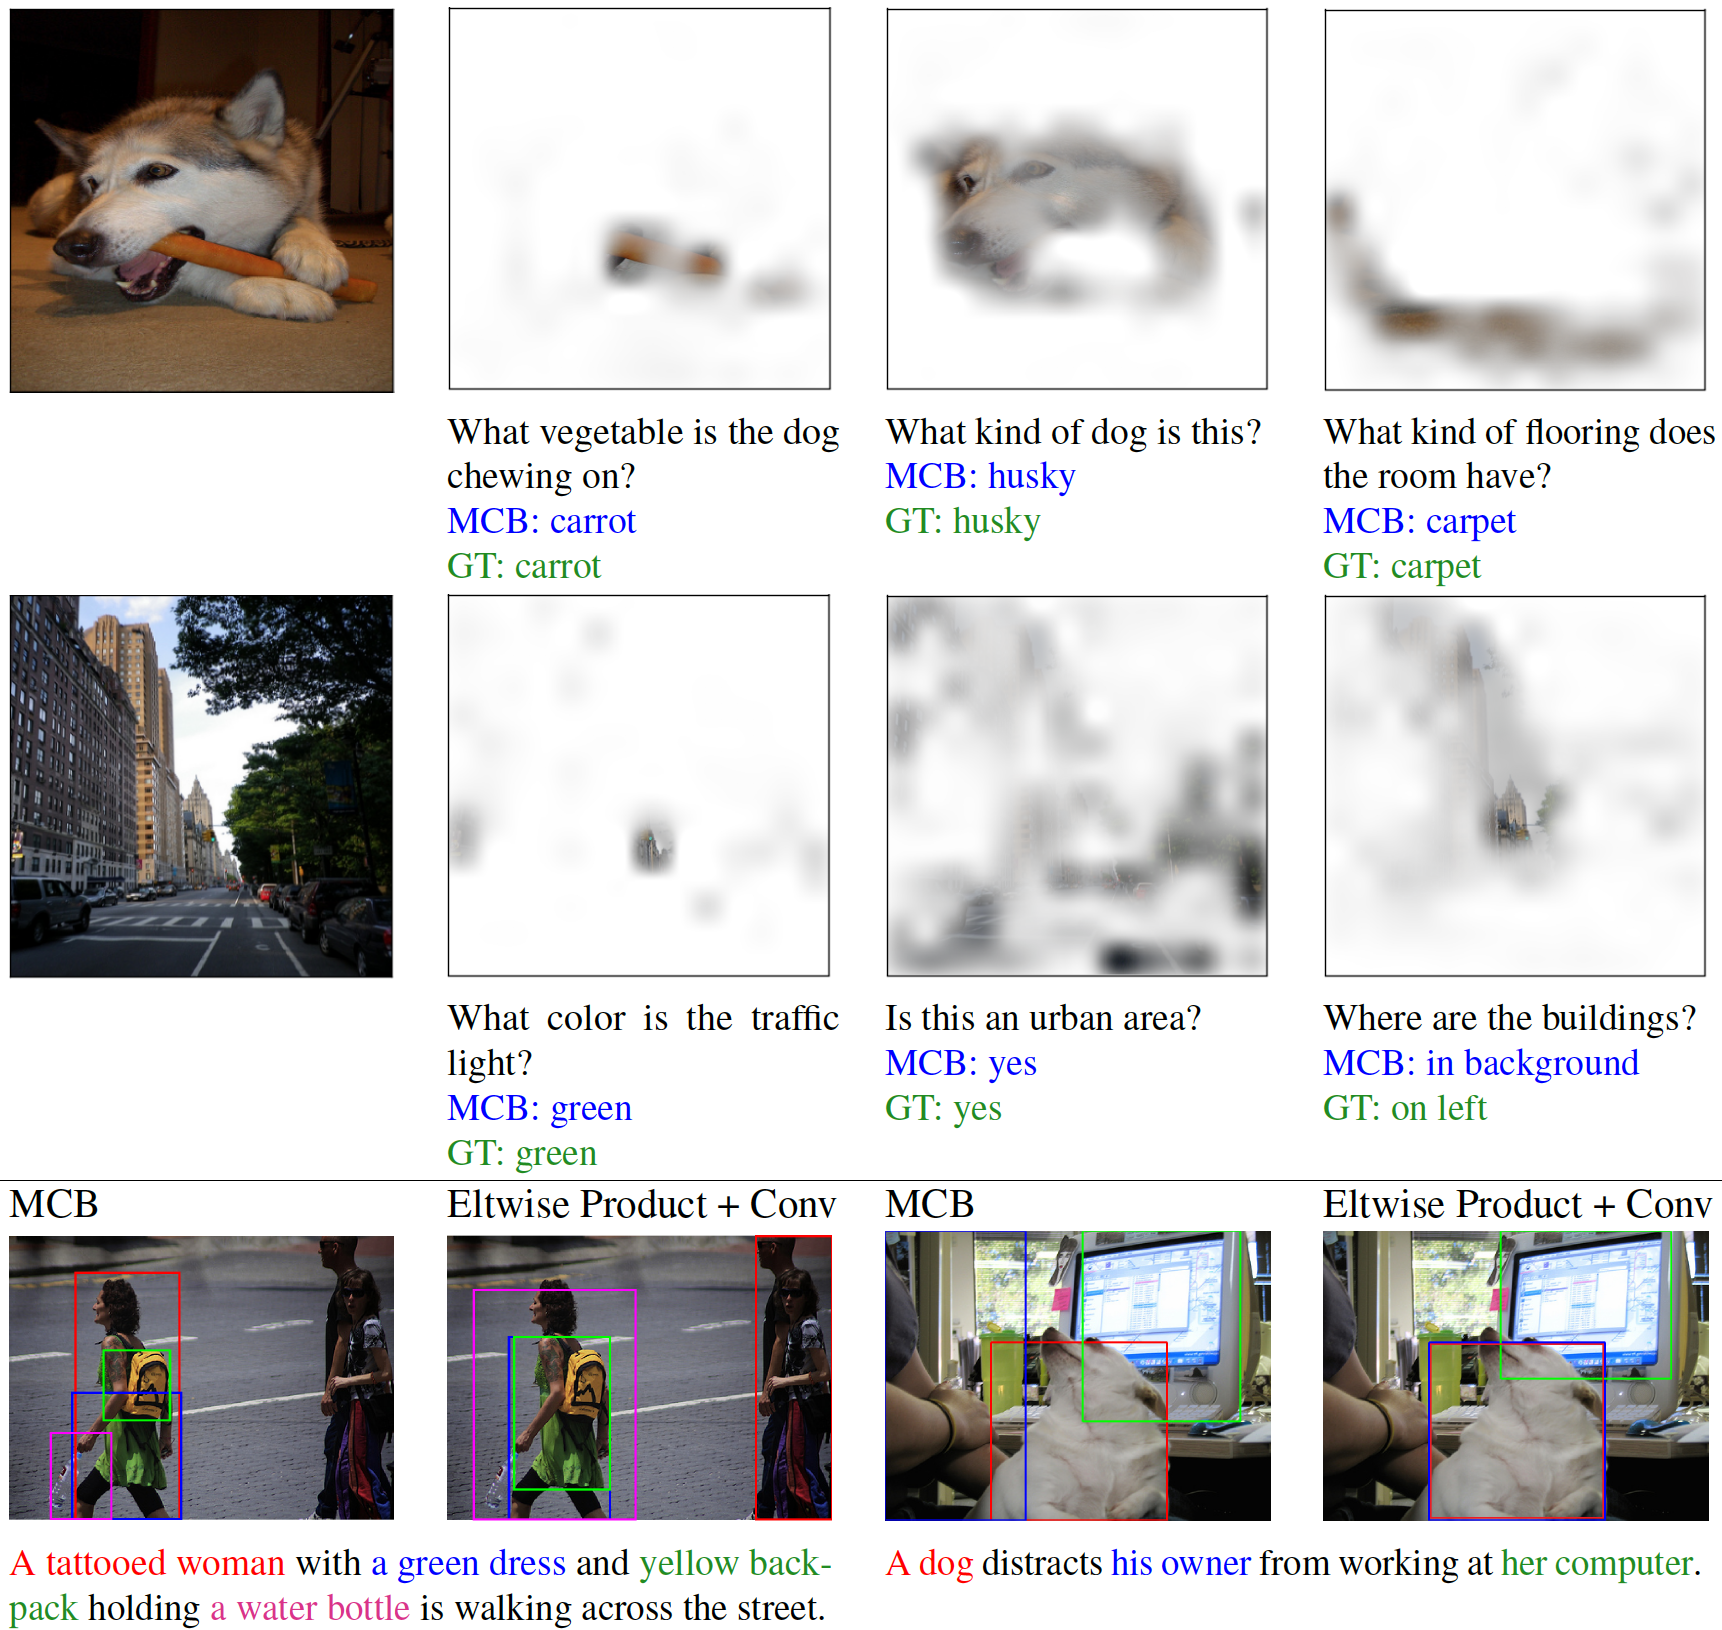
\includegraphics[scale=0.27]{./images/VG_Result02}
\end{center}
\end{frame}

%------------------------------------------------
%------------------------------------------------

\section{Conclusion} 
\begin{frame}
\frametitle{Conclusion}
\begin{itemize}
\item At the heart of MCB is the Count Sketch function
\item Count Sketch function actually limits MCB critically:
\begin{itemize}

\item  Hash collisions result in errors caused by the Count Sketch operation
\item To lower the probability of a collision, we should choose a larger counter array, 
\item For MCB to be effective, the length of the Count Sketch vector needs to be very large $(\sim16k)$.
\end{itemize}
\item \href{https://github.com/akirafukui/vqa-mcb}{The code for the paper is available in \color{blue}github} \color{black}
\end{itemize}
\end{frame}

%------------------------------------------------

\begin{frame}
\Huge{\centerline{Thank You}}
\end{frame}


%
%\begin{frame}
%\frametitle{Bullet Points}
%\begin{itemize}
%\item Lorem ipsum dolor sit amet, consectetur adipiscing elit
%\item Aliquam blandit faucibus nisi, sit amet dapibus enim tempus eu
%\item Nulla commodo, erat quis gravida posuere, elit lacus lobortis est, quis porttitor odio mauris at libero
%\item Nam cursus est eget velit posuere pellentesque
%\item Vestibulum faucibus velit a augue condimentum quis convallis nulla gravida
%\end{itemize}
%\end{frame}
%
%%------------------------------------------------
%
%\begin{frame}
%\frametitle{Blocks of Highlighted Text}
%\begin{block}{Block 1}
%Lorem ipsum dolor sit amet, consectetur adipiscing elit. Integer lectus nisl, ultricies in feugiat rutrum, porttitor sit amet augue. Aliquam ut tortor mauris. Sed volutpat ante purus, quis accumsan dolor.
%\end{block}
%
%\begin{block}{Block 2}
%Pellentesque sed tellus purus. Class aptent taciti sociosqu ad litora torquent per conubia nostra, per inceptos himenaeos. Vestibulum quis magna at risus dictum tempor eu vitae velit.
%\end{block}
%
%\begin{block}{Block 3}
%Suspendisse tincidunt sagittis gravida. Curabitur condimentum, enim sed venenatis rutrum, ipsum neque consectetur orci, sed blandit justo nisi ac lacus.
%\end{block}
%\end{frame}
%
%%------------------------------------------------
%
%\begin{frame}
%\frametitle{Multiple Columns}
%\begin{columns}[c] % The "c" option specifies centered vertical alignment while the "t" option is used for top vertical alignment
%
%\column{.45\textwidth} % Left column and width
%\textbf{Heading}
%\begin{enumerate}
%\item Statement
%\item Explanation
%\item Example
%\end{enumerate}
%
%\column{.5\textwidth} % Right column and width
%Lorem ipsum dolor sit amet, consectetur adipiscing elit. Integer lectus nisl, ultricies in feugiat rutrum, porttitor sit amet augue. Aliquam ut tortor mauris. Sed volutpat ante purus, quis accumsan dolor.
%
%\end{columns}
%\end{frame}
%
%%------------------------------------------------
%%------------------------------------------------
%
%\begin{frame}
%\frametitle{Table}
%\begin{table}
%\begin{tabular}{l l l}
%\toprule
%\textbf{Treatments} & \textbf{Response 1} & \textbf{Response 2}\\
%\midrule
%Treatment 1 & 0.0003262 & 0.562 \\
%Treatment 2 & 0.0015681 & 0.910 \\
%Treatment 3 & 0.0009271 & 0.296 \\
%\bottomrule
%\end{tabular}
%\caption{Table caption}
%\end{table}
%\end{frame}
%
%%------------------------------------------------
%
%\begin{frame}
%\frametitle{Theorem}
%\begin{theorem}[Mass--energy equivalence]
%$E = mc^2$
%\end{theorem}
%\end{frame}
%
%%------------------------------------------------
%
%\begin{frame}[fragile] % Need to use the fragile option when verbatim is used in the slide
%\frametitle{Verbatim}
%\begin{example}[Theorem Slide Code]
%\begin{verbatim}
%\begin{frame}
%\frametitle{Theorem}
%\begin{theorem}[Mass--energy equivalence]
%$E = mc^2$
%\end{theorem}
%\end{frame}\end{verbatim}
%\end{example}
%\end{frame}
%
%%------------------------------------------------
%
%\begin{frame}
%\frametitle{Figure}
%Uncomment the code on this slide to include your own image from the same directory as the template .TeX file.
%%\begin{figure}
%%\includegraphics[width=0.8\linewidth]{test}
%%\end{figure}
%\end{frame}
%
%%------------------------------------------------
%
%\begin{frame}[fragile] % Need to use the fragile option when verbatim is used in the slide
%\frametitle{Citation}
%An example of the \verb|\cite| command to cite within the presentation:\\~
%
%This statement requires citation \cite{p1}.
%\end{frame}
%
%%------------------------------------------------
%
%\begin{frame}
%\frametitle{References}
%\footnotesize{
%\begin{thebibliography}{99} % Beamer does not support BibTeX so references must be inserted manually as below
%\bibitem[Smith, 2012]{p1} John Smith (2012)
%\newblock Title of the publication
%\newblock \emph{Journal Name} 12(3), 45 -- 678.
%\end{thebibliography}
%}
%\end{frame}
%

%----------------------------------------------------------------------------------------

\end{document} 